\begin{frame}{Comparing Many Means}
    We've spent some time with hypothesis tests for 1 and 2 means... but what if we want to compare 3 or more means?
    \begin{itemize}
        \item We might think to do pairwise comparisons.
        \item However, eventually we are likely to reject $H_0$ by chance alone.
        \item We want a holistic test to examine 3 or more means.
    \end{itemize}
\end{frame}

\begin{frame}{Core Ideas of ANOVA}
    The holistic test we want is called \textbf{ANalysis Of VAriance} or \textbf{ANOVA}.
    \begin{itemize}
        \item The ANOVA tests whether means across many groups are equal.
        \item This relies on a new distribution, \textit{F}.
    \end{itemize}
\end{frame}

\begin{frame}{ANOVA Hypotheses}
    The basic hypotheses for the ANOVA are
    \begin{align*}
        H_0&: \quad \text{The mean outcome is the same across all groups.} \\
        H_A&: \quad \text{At least one mean is different.}
    \end{align*}
\end{frame}

\begin{frame}{ANOVA Hypotheses}
    In statistical notation, we write
    \begin{align*}
        H_0&: \quad \mu_1 = \mu_2 = \dots = \mu_k \\
        H_A&: \quad \mu_i \ne \mu_j \quad \text{for at least one pair } (i,j) 
    \end{align*}
    where $k$ is the number of means being compared and $i,j$ represent the $i$th and $j$th groups.
\end{frame}

\begin{frame}{ANOVA Assumptions}
    There are three core conditions for ANOVA:
    \begin{enumerate}
        \item Observations independent within and between groups.
        \item Data within each group are nearly normal.
        \item Variability across groups is about equal.
    \end{enumerate}
\end{frame}

\begin{frame}{Example}
    \begin{itemize}
        \item A university offers 3 lectures for an introductory psychology course.
        \item A single professor offers 8am, 10am, and 3pm lectures.
        \item We want to know if the average midterm scores differ between these lectures.
    \end{itemize}
    Describe appropriate hypotheses to determine whether there are any differences between the three classes.
\end{frame}

\begin{frame}{Why "Analysis of Variance"?}
    \begin{itemize}
        \item Strong evidence favoring $H_A$ will be unusually large differences between group means. 
        \item It may come as a surprise, but we will quantify this by examining variability.
    \end{itemize}
\end{frame}

\begin{frame}{Example: High Within Group Variance}
    \begin{figure}
        \centering
        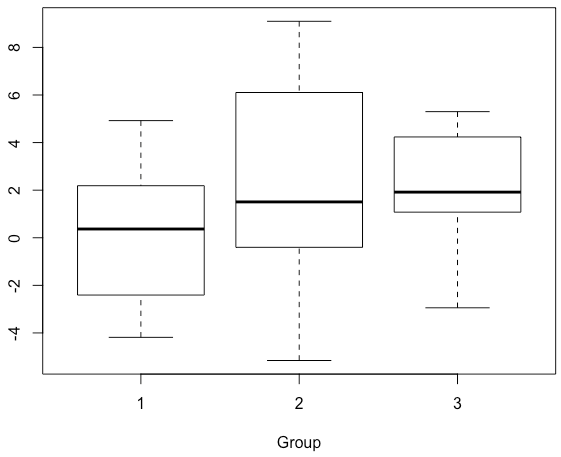
\includegraphics[height=3in]{images/highvar.png}
    \end{figure}
\end{frame}

\begin{frame}{Example: Low Within Group Variance}
    \begin{figure}
        \centering
        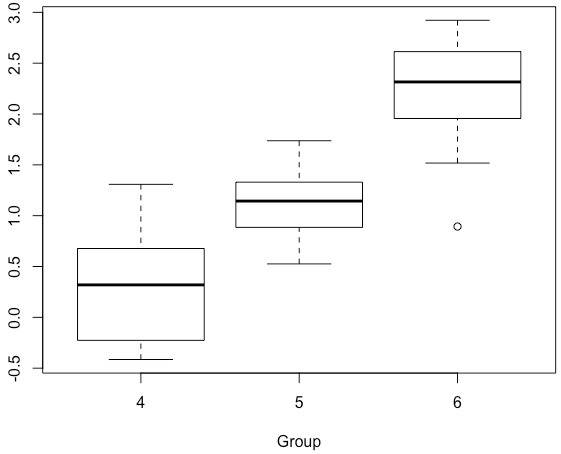
\includegraphics[height=3in]{images/lowvar.png}
    \end{figure}
\end{frame}

\begin{frame}{Example: All 6 Groups}
    \begin{figure}
        \centering
        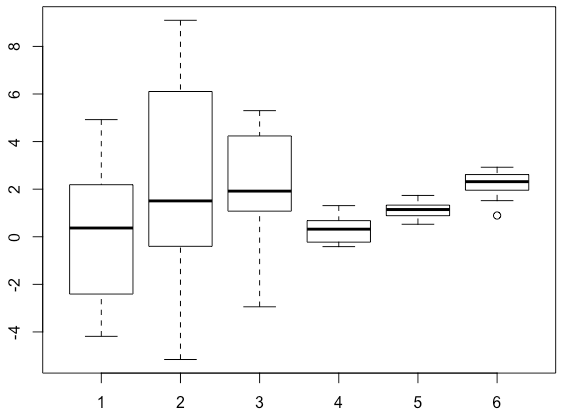
\includegraphics[height=3in]{images/bothvar.png}
    \end{figure}
\end{frame}

\begin{frame}{Why "Analysis of Variance"?}
    \begin{itemize}
        \item We were able to see the differences in groups 4, 5, and 6 more easily.
        \item The differences in center are more obvious because the differences are large \textit{relative to the within group variability}.
    \end{itemize}
\end{frame}

\begin{frame}{Example: MLB Batting Performance and Player Position}
    \begin{itemize}
        \item We want to determine whether batting performance differs between positions (outfielder, infielder, and catcher).
        \item We have a dataset from 2018 with batting records of 429 MLB players.
        \item We will compare on-base percentage, roughly the fraction of times a player gets on base or hits a home run.
    \end{itemize}
\end{frame}

\begin{frame}{Example: MLB}
    \begin{table}
        \centering%\small
        \begin{tabular}{r llll}
            \hline
            & Name & Team & Position & OBP \\ 
            \hline
            1 & Abreu, J & CWS & IF & 0.325 \\
            2 & Acuna Jr., R & ATL & OF & 0.366\\
            3 & Adames, W & TB & IF & 0.348 \\
            \vdots & \vdots & \vdots & \vdots & \vdots \\
            427 & Zimmerman, R & WSH & IF & 0.337 \\
            428 & Zobrist, B & CHC & IF & 0.378 \\
            429 & Zunino, M & SEA & C & 0.259 \\
             \hline
        \end{tabular}
    \end{table}
\end{frame}

\begin{frame}{Example: MLB}
    Write the null and alternative hypotheses.
\end{frame}

\begin{frame}{Example: MLB}
    The by-group summary statistics are
    \begin{table}[]
        \centering%\small
        \begin{tabular}{l rrr}
            \hline
            & OF & IF & C \\
            \hline
            Sample size ($n_i$) & 160 & 205 & 64 \\
            Sample mean ($\bar{x}_i$) & 0.320 & 0.318 & 0.302 \\
            Sample sd ($s_i$) & 0.043 & 0.038 & 0.038 \\
            \hline
        \end{tabular}
    \end{table}
\end{frame}

\begin{frame}{Example: MLB}
    \begin{center}
        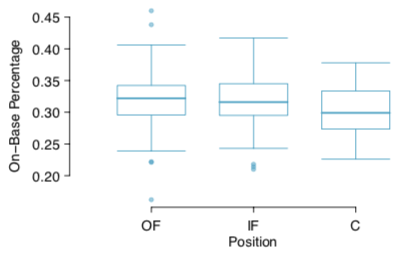
\includegraphics[height=2in]{images/mlb.png}
    \end{center}
\end{frame}

\begin{frame}{Example: MLB}
    \begin{itemize}
        \item The largest difference is between the OF and C groups.
        \item Why not just run a test of $H_0:$ $\mu_{OF} = \mu_C$?
        \begin{itemize}
            \item We may miss differences between $\mu_{OF}$ and $\mu_{IF}$ or $\mu_{C}$ and $\mu_{IF}$.
            \item We are inspecting the data before picking comparison groups.
        \end{itemize}
    \end{itemize}
\end{frame}

\begin{frame}{Example}
    Informal testing (looking at graphs or summary statistics) before choosing tests is called \textbf{data snooping}, \textbf{data fishing}, or \textbf{data hacking}.
    \begin{itemize}
        \item This will inflate the Type I error rate.
    \end{itemize}
\end{frame}

\begin{frame}{Multiple Comparisons and Type I Error}
\begin{center}
    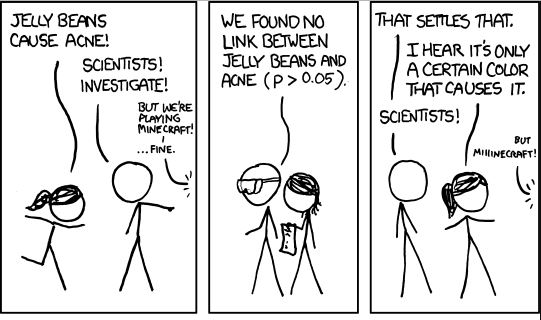
\includegraphics[height=2in]{images/xkcd1.JPG}
\end{center}
\hfill\flushright\tiny
Source: xkcd "Significant" (https://xkcd.com/882/)
\end{frame}

\begin{frame}{Multiple Comparisons and Type I Error}
\begin{center}
    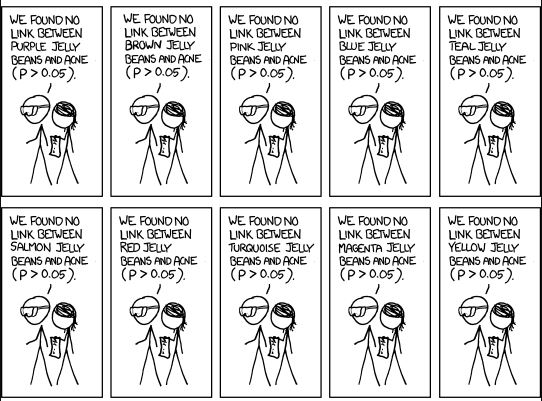
\includegraphics[width=3.5in]{images/xkcd2.JPG}
\end{center}
\flushright\tiny
Source: xkcd "Significant" (https://xkcd.com/882/)
\end{frame}

\begin{frame}{Multiple Comparisons and Type I Error}
\begin{center}
    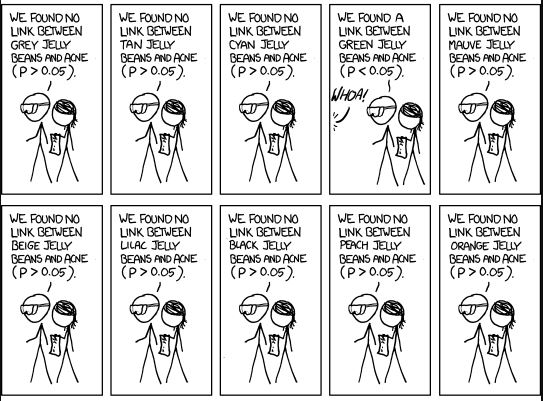
\includegraphics[width=3.5in]{images/xkcd3.JPG}
\end{center}
\flushright\tiny
Source: xkcd "Significant" (https://xkcd.com/882/)
\end{frame}

\begin{frame}{Multiple Comparisons and Type I Error}
\begin{center}
    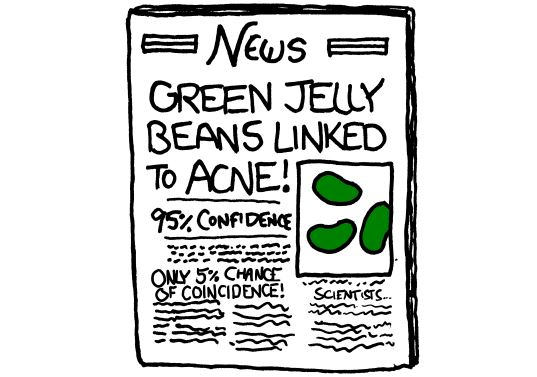
\includegraphics[height=2in]{images/xkcd4.JPG}
\end{center}
\hfill\flushright\tiny
Source: xkcd "Significant" (https://xkcd.com/882/)
\end{frame}

\begin{frame}{The F Distribution}
    \begin{center}
        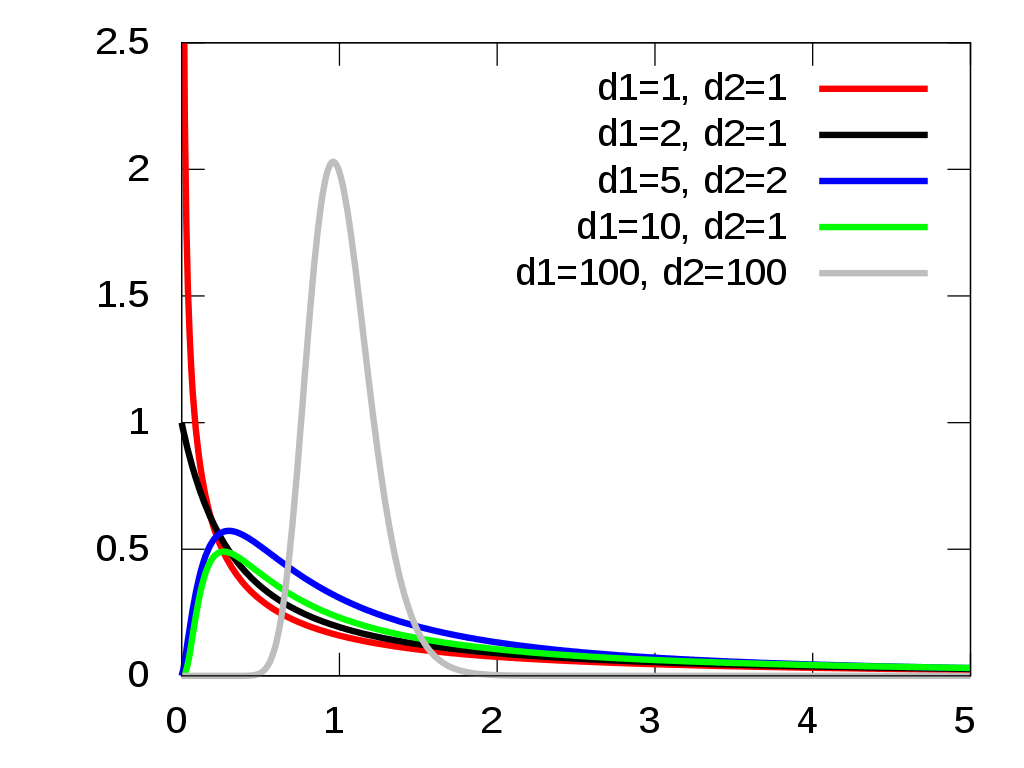
\includegraphics[height=2.5in]{images/fdist.png}
    \end{center}
\end{frame}

\begin{frame}{The F Distribution}
    The F distribution...
    \begin{itemize}
        \item Only takes values $\ge 0$.
        \item Is always right skewed.
        \item Depends on two sets of degrees of freedom ($df_1$ and $df_2$). 
    \end{itemize}
    
    \vspace{12pt}
    We say $X \sim F(df_1,$ $df_2$).
\end{frame}

\begin{frame}{The F Distribution}
    The F distribution can be written as the \textit{ratio of two variances}.
    \[
        \frac{s_1/df_1}{s_2/df_2}
    \]
    will have an $F(df_1, df_2)$ distribution. 
\end{frame}

\begin{frame}{ANOVA and the F-test}
    \begin{itemize}
        \item Question: is the variability in the sample means so large that it seems unlikely to be from chance alone?
        \item We call this variability the \textbf{mean square between groups} (MSG) or \textbf{mean square for treatment} (MST).
    \end{itemize}
\end{frame}

\begin{frame}{Mean Square Between Groups}
    \begin{itemize}
        \item This acts as a measure of variability for the $k$ group means.
        \item It has degrees of freedom $df_G = k-1$.
        \item If $H_0$ is true, we expect this variability to be small.
    \end{itemize}
\end{frame}

\begin{frame}{Mean Square Between Groups}
    \begin{align*}
        MSG &= \frac{1}{df_G}SSG \\
        &= \frac{1}{k-1}\sum_{i=1}^{k}(\bar{x}_i - \bar{x})^2
    \end{align*}
    where SSG is the sum of squares between groups.
\end{frame}

\begin{frame}{Mean Square Between Groups}
    \begin{figure}
        \centering
        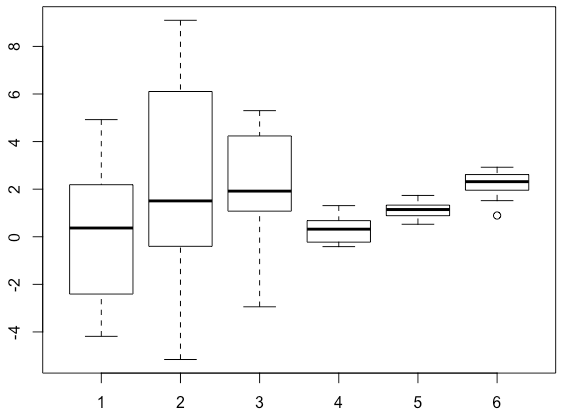
\includegraphics[height=2.5in]{images/bothvar.png}
    \end{figure}
    ...but MSG isn't very useful on its own.
\end{frame}

\begin{frame}{Mean Square Error}
    \begin{itemize}
        \item We need an idea of how much variability would be expected (or normal) if $H_0$ were true.
        \item This is done using a pooled variance estimate, called the \textbf{mean square error} (MSE).
        \item This is a measure of variability within groups.
        \item MSE has degrees of freedom $df_E = n-k$
    \end{itemize}
\end{frame}

\begin{frame}{Mean Square Error}
    \begin{align*}
        MSE &= \frac{1}{df_E}SSE \\
        &= \frac{1}{n-k}\sum_{i=1}^k (n_i - 1)s_i^2
    \end{align*}
    where SSE is the sum of squares for error and $s_i$ is the standard deviation for the observations in group $i$.
\end{frame}

\begin{frame}{Sum of Squares Total}
    It's also useful to think of a \textbf{sum of squares total} (SST)
    \begin{align*}
        SST &= SSG + SSE
    \end{align*}
    and total degrees of freedom
    \begin{align*}
        df_T &= df_G + df_E \\
        &= k-1 + n-k \\ 
        &= n-1
    \end{align*}
\end{frame}

\begin{frame}{Mean Square Total}
    If we were to find the mean square total,
    \begin{align*}
        MST &= \frac{1}{df_T}SST \\
        &= \frac{1}{n-1}(SSG + SST) \\
        &= \frac{1}{n-1}\sum_{j=1}^n(x_i - \bar{x})^2
    \end{align*}
    we would get the variance across all observations!
\end{frame}

\begin{frame}{ANOVA}
    The ANOVA breaks the variance down into 
    \begin{itemize}
        \item within group (random) variability (MSE).
        \item between group (means) variability (MSG).
    \end{itemize}
\end{frame}

\begin{frame}{ANOVA}
    We want to know how much variability is due to differences in groups \textit{relative to the within groups variability}. 
    
    \vspace{12pt}So our test statistic is
    \[
        F = \frac{MSG}{MSE}
    \]
\end{frame}

\begin{frame}{Example}
    For our baseball example,
    \begin{table}[]
        \centering%\small
        \begin{tabular}{l rrr}
            \hline
            & OF & IF & C \\
            \hline
            Sample size ($n_i$) & 160 & 205 & 64 \\
            Sample mean ($\bar{x}_i$) & 0.320 & 0.318 & 0.302 \\
            Sample sd ($s_i$) & 0.043 & 0.038 & 0.038 \\
            \hline
        \end{tabular}
    \end{table}
    $MSG=0.00803$ and $MSE = 0.00158$. 
    
    \vspace{12pt}
    Find the degrees of freedom and the F statistic. 
\end{frame}

\begin{frame}{The F Test}
    With our F distribution comes the \textbf{F-test}. Using the F-distribution, we calculate
    \begin{itemize}
        \item $F_{\alpha}(df_1,df_2)$ critical values.
        \item p-values
    \end{itemize}
\end{frame}

\begin{frame}{The F Test}
    If the between-group variability is high relative to the within group variability,
    \begin{itemize}
        \item $MSG > MSE$
        \item F will be large.
        \item Large values of F represent stronger evidence against the null.
    \end{itemize}
\end{frame}

\begin{frame}{The F Test}
    This is the F(2, 426) distribution from our baseball example.
    \begin{center}
        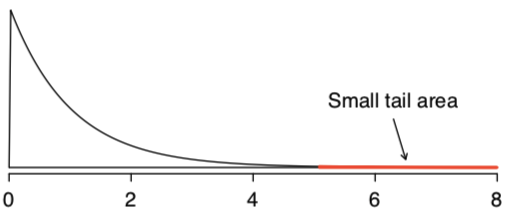
\includegraphics[width=3.5in]{images/fdistbaseball.png}
    \end{center}
    
    \begin{itemize}
        \item F-test p-values will always be from the upper tail area.
        \item We no longer have one- or two-sided tests to worry about.
        \item The critical value is $F_{0.05}(2, 426) = 3.0169$.
    \end{itemize}
\end{frame}

\begin{frame}{Example}
    What can we conclude about the baseball field positions?
    
    \vspace{12pt}Recall $F_{0.05}(2, 426) = 3.0169$.
\end{frame}

\begin{frame}{Reading an ANOVA Table}
    \begin{itemize}
        \item Typically we will run ANOVA using software.
        \item Fortunately there is a standard output for this analysis.
    \end{itemize}
    
    \vspace{12pt}Let's take some time to write out the ANOVA table.
\end{frame}

\begin{frame}{Reading an ANOVA Table from Software}
    This is the ANOVA from \texttt{R} for the MLB example. 
    \begin{table}[]
        \centering{\setlength{\extrarowheight}{10pt}
        \begin{tabular}{l ccccc}
            \hline
             & Df & Sum Sq & Mean Sq & F value & Pr($>$F)\\
            \hline
            position & 2 & 0.0161 & 0.0080 & 5.0766 & 0.0066 \\
            Residuals & 426 & 0.6740 & 0.0016 & & \\
            \hline
        \end{tabular}}
    \end{table}
    What can we conclude based on the table?
\end{frame}

\begin{frame}{Example}
    Suppose we have 10 data points from each of 5 groups of interest.
    \begin{table}[]
        \centering{\setlength{\extrarowheight}{10pt}
        \begin{tabular}{l cccc}
            \hline
            Source      & df & SS & MS & F  \\
            \hline
            Group       & \rule{1cm}{0.15mm} & \rule{1cm}{0.15mm}  & 3 & \rule{1cm}{0.15mm} \\
            Error   & \rule{1cm}{0.15mm} & \rule{1cm}{0.15mm}  & \rule{1cm}{0.15mm} & \\
            Total       & \rule{1cm}{0.15mm} & 20 &  & \\
            \hline
        \end{tabular}}
    \end{table}
    Fill in the missing information from the ANOVA table.
\end{frame}

\begin{frame}{Graphical Diagnostics for ANOVA}
    There are three conditions for ANOVA:
    \begin{enumerate}
        \item Independence
        \item Approximate normality
        \item Constant variance
    \end{enumerate}
\end{frame}

\begin{frame}{ANOVA Diagnostics: Independence}
    \begin{itemize}
        \item It is reasonable to assume independence if the data are a simple random sample.
        \item If the data are not a random sample, consider carefully.
        \begin{itemize}
            \item In the MLB example, no clear reason why a player's batting stats would impact another player's batting stats.
        \end{itemize}
    \end{itemize}
\end{frame}

\begin{frame}{ANOVA Diagnostics: Normality}
    \begin{center}
        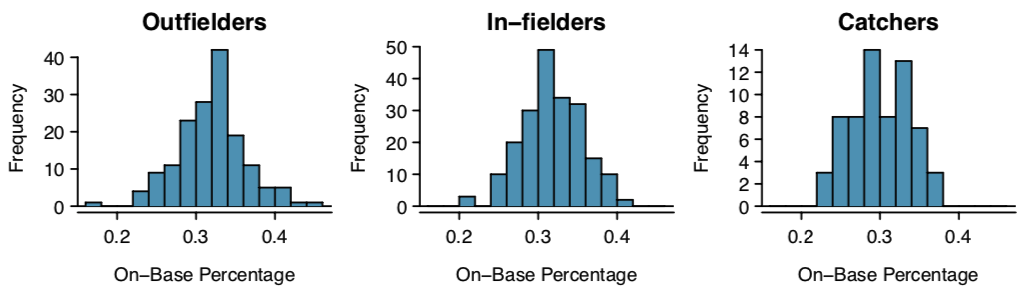
\includegraphics[width=4in]{images/obphists.png}
    \end{center}
    \begin{itemize}
        \item Normality is especially important for small samples.
        \item For large samples, ANOVA is \textit{robust to} deviations from normality.
    \end{itemize}
\end{frame}

\begin{frame}{ANOVA Diagnostics: Constant Variance}
    \begin{center}
        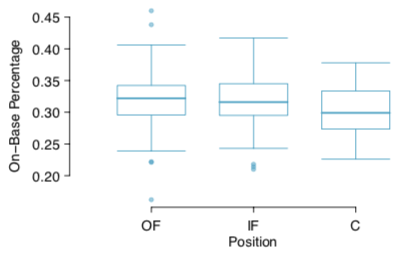
\includegraphics[width=3in]{images/mlb.png}
    \end{center}
    \vspace{-12pt}\begin{itemize}
        \item We can check this visually or by examining the standard deviations for each group.
        \item Constant variance is especially important when the sample sizes differ between groups.
    \end{itemize}
\end{frame}

\begin{frame}{After the ANOVA}
    For an ANOVA,
    \begin{align*}
        H_0&: \quad \mu_1 = \mu_2 = \dots = \mu_k \\
        H_A&: \quad \mu_i \ne \mu_j \quad \text{for at least one pair } (i,j) 
    \end{align*}
    If we reject $H_0$, we know that at least one mean differs... but we don't know where those differences lie.
\end{frame}

\begin{frame}{Multiple Comparisons}
    Consider an ANOVA with three groups. If we reject $H_0$, there are three comparisons to make:
    \begin{itemize}
        \item group 1 and group 2
        \item group 1 and group 3
        \item group 2 and group 3
    \end{itemize}
\end{frame}

\begin{frame}{Multiple Comparisons}
    Most of this builds on techniques you already know!
    \begin{itemize}
        \item We compare groups using a two-sample t-test.
        \item But we need to modify the significance level.
        \item We also use a pooled standard deviation estimate.
    \end{itemize}
\end{frame}
%Usually this pooled standard deviation can be found in the ANOVA table, e.g. along the bottom of Figure 7.25.

\begin{frame}{Example}
    \begin{itemize}
        \item A university offers 3 lectures for an introductory psychology course.
        \item A single professor offers 8am, 10am, and 3pm lectures.
        \item We want to know if the average midterm scores differ between these lectures.
    \end{itemize}
    We already wrote down hypotheses for this ANOVA. 
\end{frame}

\begin{frame}{Example}
    Are the ANOVA conditions satisfied?
    \begin{columns}\begin{column}{0.4\textwidth}
        \small{\begin{tabular}{l ccc}
            \hline
            Class $i$ & A & B & C \\
            \hline
            $n_i$ & 58 & 55 & 51 \\
            $\bar{x}_i$ & 75.1 & 72.0 & 78.9 \\
            $s_i$ & 13.8 & 13.9 & 13.1 \\
            \hline
        \end{tabular}}
    \end{column}\begin{column}{0.6\textwidth}
        \begin{center}
            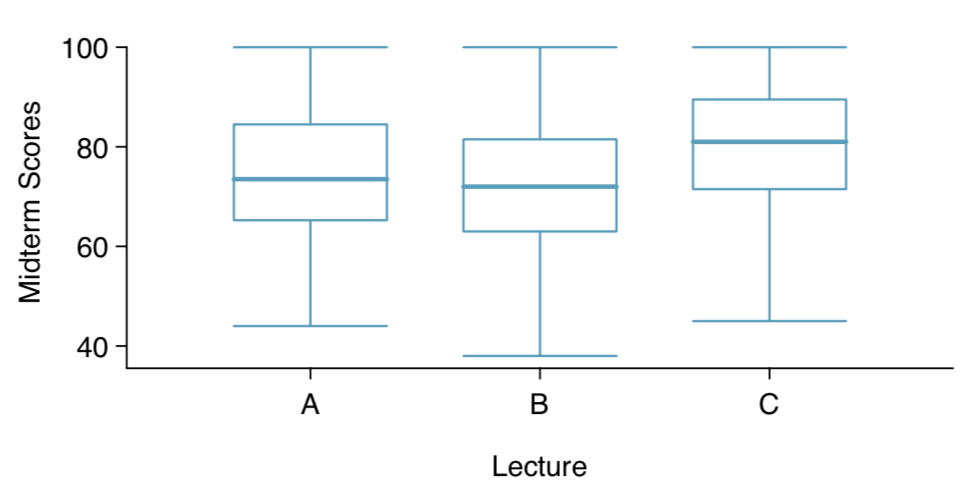
\includegraphics[scale=0.4]{images/examboxplts.png}
        \end{center}
    \end{column}\end{columns}
\end{frame}

\begin{frame}{Example}
    Here is part of the ANOVA for this data (\texttt{R} output):
    \begin{table}[]
        \centering
        \begin{tabular}{l rrrrr}
            \hline
             & Df & Sum Sq & Mean Sq & F value & Pr($>$F) \\
            \hline
            lecture     & & & 645.06 & & 0.0330 \\
            Residuals   & & & 185.16 & & \\
            \hline
        \end{tabular}
    \end{table}
    Let's fill in the rest. What can we conclude?
\end{frame}

\begin{frame}{Example}
    So at least one pair of means differ... but which?
    \begin{itemize}
        \item We need to correct for Type I error before running our t-tests.
    \end{itemize}
\end{frame}

\begin{frame}{Pooled Standard Error}
    Pooled standard error may be calculated as follows:
    \[
        s_{pooled} = \sqrt{\frac{(n_1-1)s_1^2 + (n_2-1)s_2^2 + \dots + (n_k-1)s_k^2}{n - k}}
    \]
    where $n = n_1 + n_2 + \dots + n_k$ is the total number of observations.
\end{frame}

\begin{frame}{Pooled Standard Error}
    If each group's sample size is equal,
    \[
        s_{pooled} = \sqrt{\frac{s_1^2 + s_2^2 + \dots + s_k^2}{k}}
    \]
    
    The degrees of freedom for these t-tests will be $n-k$.
\end{frame}

\begin{frame}{Example}
    \begin{table}[]
        \centering
        \begin{tabular}{l ccc}
            \hline
            Class $i$ & A & B & C \\
            \hline
            $n_i$ & 58 & 55 & 51 \\
            $\bar{x}_i$ & 75.1 & 72.0 & 78.9 \\
            $s_i$ & 13.8 & 13.9 & 13.1 \\
            \hline
        \end{tabular}
    \end{table}
    Let's calculate the pooled standard error for our exams.
\end{frame}

\begin{frame}{Example}
    \texttt{R} also provides the pooled standard deviation estimate with the ANOVA output.
    \begin{table}[]
        \centering
        \begin{tabular}{l rrrrr}
            \hline
             & Df & Sum Sq & Mean Sq & F value & Pr($>$F) \\
            \hline
            lecture     & 2   & 1290.11 & 645.06 & 3.48 & 0.0330 \\
            Residuals   & 161 & 29810.12 & 185.16 & & \\
            \hline
             & & & \multicolumn{3}{r}{$s_{pooled} = 13.61$ on $df=161$}
        \end{tabular}
    \end{table}
\end{frame}

\begin{frame}{Significance Level Adjustments}
    \begin{itemize}
        \item The final adjustment is to modify the significance level.
        \item When we do many pairwise comparisons, we increase our chances of Type I error.
        \item This correction will adjust our probability of Type I error.
        \item Adjusted significance levels will help ensure that the Type I error is no greater than $\alpha$.
    \end{itemize}
\end{frame}

\begin{frame}{The Bonferroni Correction}
    Testing many pairs of groups is called \textbf{multiple comparisons}. The \textbf{Bonferroni correction} sets a new significance level $\alpha^*$:
    \[
        \alpha^* = \alpha/K
    \]
    where $K$ is the number of comparisons. 
\end{frame}

\begin{frame}{Example}
    Complete the pairwise comparisons for the three lectures.
\end{frame}

\begin{frame}{Post ANOVA: Other Situations}
    If we fail to reject $H_0$ in an ANOVA
    \begin{itemize}
        \item No pairwise comparisons are necessary.
        \item (None will be significant.)
    \end{itemize}
    
    \vspace{12pt}If we reject $H_0$ in an ANOVA
    \begin{itemize}
        \item Sometimes our pairwise comparisons won't show any significance.
        \item This does not invalidate the ANOVA results!
    \end{itemize}
\end{frame}

\begin{frame}{Multiple Comparisons}
    The Bonferroni correction is one method of many! Others include
    \begin{itemize}
        \item Tukey's Honest Significant Difference
        \item Scheffe's Method
        \item and others.
    \end{itemize}{}
    We will not learn these in detail.
\end{frame}
